\documentclass[a4paper]{article}

\usepackage{graphicx}
\usepackage{float}
\usepackage{hyperref}
\usepackage{xcolor}
\usepackage[spanish]{babel}
\usepackage{listings}
\usepackage{enumitem}
\usepackage[utf8]{inputenc}

\lstset{language=c, frame=tlrb, basicstyle=\scriptsize, breaklines=true, numberbychapter=false,numbers=left}
\setlist[enumerate]{noitemsep}
\setlist[itemize]{noitemsep}

\begin{document}

\title{Infraestructura de Análisis de Rendimiento\\
\bigskip
{\large Propuesta de tesis para\\} Magister en Cómputo de Altas Prestaciones\\
\bigskip
Universidad Nacional de La Plata\\
Facultad de Informática\\
\bigskip
}

\author{Tesista: Andrés More - {\tt amore@hal.famaf.unc.edu.ar}\\
Director: Dr. Fernando G. Tinetti - {\tt fernando@lidi.info.unlp.edu.ar}}

\date{Octubre de 2013}

\maketitle

\newpage

\section{Objetivo}

La propuesta principal consiste en el desarrollo de una infraestructura de soporte para el análisis de aplicaciones de Cómputo de Altas Prestaciones. Este trabajo se realiza en continuación al trabajo final {\it Herramientas para el Soporte de Análisis de Rendimiento} de la Especialización en Cómputo de Altas Prestaciones y Tecnología Grid.

\bigskip

La infraestructura implementará una serie de etapas donde se automatiza un proceso de análisis de rendimiento ejecutando pruebas de referencia, herramientas de perfil de rendimiento y análisis de resultados. Luego se genera un reporte que soporta el análisis de rendimiento con información cuantitativa.
Se incluirá datos estadísticos de la aplicación y el sistema donde se ejecuta, además de gráficos de desviación, escalamiento de problemas y cómputo e identificación de cuellos de botella.

\section{Motivación/Estado del Arte del Tema}

En el área de cómputo de altas prestaciones los desarrolladores son los mismos
especialistas del dominio del problema a resolver. Las rutinas
más demandantes de cálculo son en su mayoría científicas y su
alta complejidad hace posible su correcta implementación sólo por los mismos investigadores.

\bigskip

Estas cuestiones resultan en un tiempo reducido de optimización de rendimiento
e impactan directamente en la productividad de los grupos de investigación y
desarrollo. Frecuentemente el proceso de optimización termina siendo
hecho de modo {\it ad-hoc}, sin la utilización de información cuantitativa para dirigir los
esfuerzos de optimización.

\bigskip

Algunas referencias a la problemática se incluyen a continuación como soporte de la propuesta:

\begin{itemize}

\item Como correctamente mostrar resultados de rendimiento por {\it Fleming, Philip J. and Wallace, John J.} en {\it How Not to Lie with Statistics: the Correct Way to Summarize Benchmark Results}, {ACM}, {29/3}, {1986}.

\item Como acceder a memoria eficientemente por {\it Drepper, Ulrich} en {\it What Every Programmer Should Know About Memory}, Reporte Técnico, 2007.

\item Una discusión de la dificultad de la programación en paralelo por {\it McKenney, Paul E.} en {\it Is Parallel Programming Hard, And, If So, What Can You Do About It?}, Reporte Técnico, 2007.

\item Una revisión de como medir rendimiento durante el desarrollo de una aplicación por {\it Woodside, Murray and Franks, Greg and Petriu, Dorina C.} en {\it The Future of Software Performance Engineering}, IEEE Computer Society, 2007.

\end{itemize}

\section{Temas de Investigación}

Esta sección contiene una lista inicial de los temas a desarrollar.

\begin{enumerate}
\item Automatización de ejecución de pruebas de referencia
\item Aplicación general de herramientas de perfil de ejecución
\item Generación de gráficos de rendimiento
\item Generación de reportes
\end{enumerate}

\section{Desarrollos/Trabajo Experimental a Realizar}

La infraestructura a desarrollar consiste de distintos componentes, como se demuestra en la Figura \ref{fig:framework} a continuación.

\begin{figure}[H]
\centering
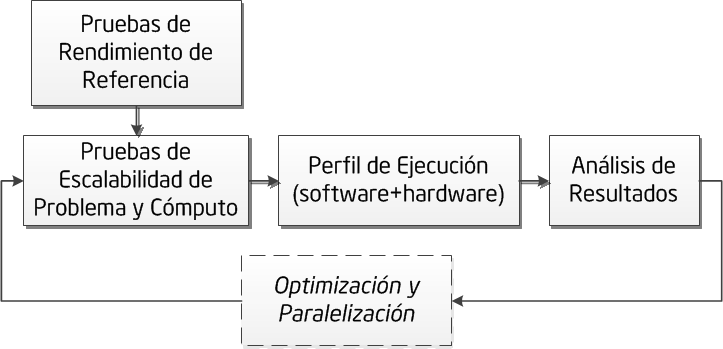
\includegraphics{framework.png}
\caption{Infrastructura a Desarrollar}
\label{fig:framework}
\end{figure}

  \begin{description}
  \item[Ejecución de pruebas de rendimiento:] automáticamente configura y ejecuta pruebas, publicando números de rendimiento relevantes.
  \item[Aplicación de herramientas de soporte:] automáticamente configura y ejecuta herramientas para medir rendimiento e identificar cuellos de botella.
  \item[Análisis de datos de rendimiento:] utilizando la información anterior, calcula límites de potenciales mejoras y lista los cuellos de botella principales.
  \item[Generación de reporte:] a partir de la información anterior, compila un reporte incluyendo gráficos y referencias al código específico a optimizar.
  \end{description}

\section{Esquema de Plan de Trabajo}

El siguiente cronograma muestra el plan de actividades tentativo incluyendo actividades y tiempos.

\begin{table}[H]
  \caption{Detalle de Actividades}
  \centering
    \begin{tabular}{|l|l|}\hline
      {\bf Actividad} & {\bf Duración} \\ \hline
      Diseño de Alto Nivel & Noviembre \\ \hline
      Prototipo & Diciembre-Enero-Febrero \\ \hline
      Pruebas de Rendimiento & Marzo \\ \hline
      Cálculo de Leyes & Abril \\ \hline
      Perfil de Rendimiento & Mayo-Junio-Julio \\ \hline
      Eventos y Vectorización & Agosto \\ \hline
      Realización Tesis & Septiembre-Octubre \\ \hline
    \end{tabular}
  \label{schedule}
\end{table}

\section{Posibilidades de Realización}

El alumno tiene a su disposición acceso al equipamiento necesario como parte de su ámbito laboral.
El alumno trabaja como Ingeniero en Software en {\it Argentina Software Design Center} (ASDC - Intel Córdoba); también
como docente e investigador en el Instituto Universitario Aeronáutico dictando tanto cursos de grado (Cómputo de Altas Prestaciones) como postgrado (Implementación de Sistemas Operativos).

\section{Bibliografía Básica Relacionada}

Un conjunto inicial a modo de referencia es incluido en la bibliografía listada a continuación.

\begin{thebibliography}{9}
  
\bibitem{critical-overview}
 J. Browne,
 \emph{A critical overview of computer performance evaluation},
 1976.

\bibitem{patterns}
 G. Mattson, B.A. Sanders and B.L. Massingill, 
 \emph{Patterns for Parallel Programming, Addison-Wesley},
 2004.

\bibitem{automatic-performance-analysis}
 T. Margalef, J. Jorba, O. Morajko, A. Morajko, E. Luque,
 \emph{Different approaches to automatic performance analysis of distributed applications},
 2004.

\bibitem{intro-software-performance}
 C. Smith,
 \emph{Introduction to software performance engineering: origins and outstanding problems},
 2007.

\bibitem{future-software-performance}
 M. Woodside, G. Franks, D. Petriu,
 \emph{The Future of Software Performance Engineering},
 2007.

\bibitem{capturing-performance-knowledge}
 K. Huck, O. Hernandez, V. Bui, S. Chandrasekaran, B. Chapman, A. Malony, L McInnes, B. Norris,
 \emph{Capturing performance knowledge for automated analysis},
 2008.

\bibitem{spec}
  Andres More,
 \emph{Herramientas de Soporte para Análisis de Rendimiento},
 Trabajo Final Especializacion HPC/GRID - UNLP 2013.

\bibitem{counters}
  Fernando G. Tinetti, Mariano Mendez, and Armando De Giusti,
  \emph{An Automated Approach to Hardware Performance Monitoring Counters},
  2013. 

\end{thebibliography}

\end{document}
